\chapter{Запаздывание}
\label{ch:chap3}

В соответствии с моим вариантом:
$$
    j=2, \tab W_3(s) = \frac{7s+5}{s^2 + 4s}, \tab W_4(s) = \frac{20s^2 +1.6s +2}{10s^3-10s^2-0.1s+0.1}
$$
Необходимо добавить к каждой ПФ звено чистого запаздывания $e^{-\tau s}$.

\section{Передаточная функция $W_3$}

Рассмотрим обновлённую ПФ:
$$
    W_3(s) = \frac{7s+5}{s^2 + 4s}e^{-\tau s}
$$
Получаем её полюса: $\lambda_{1,2} = \{-4, 0\}$, система имеет два устойчивых полюса.

Построим для неё годографы, с разными $\tau$:
\begin{figure}[ht]
    \centering
    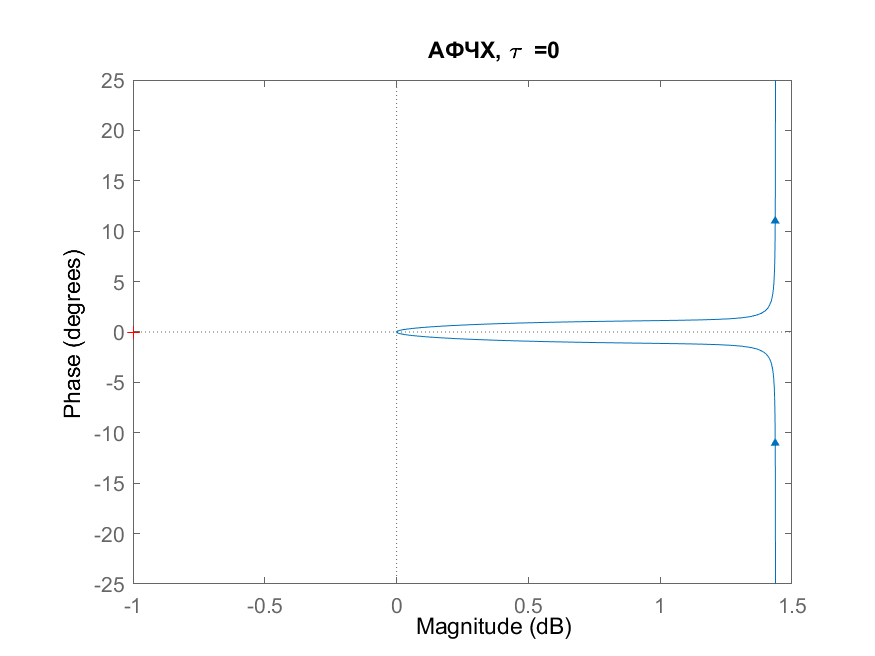
\includegraphics[width=0.7\textwidth]{nyquist_task31_object1.png}
    \caption{Годограф Найквиста для разомкнутой системы, $\tau=0$}
\end{figure}
\newpage
\begin{figure}[ht]
    \centering
    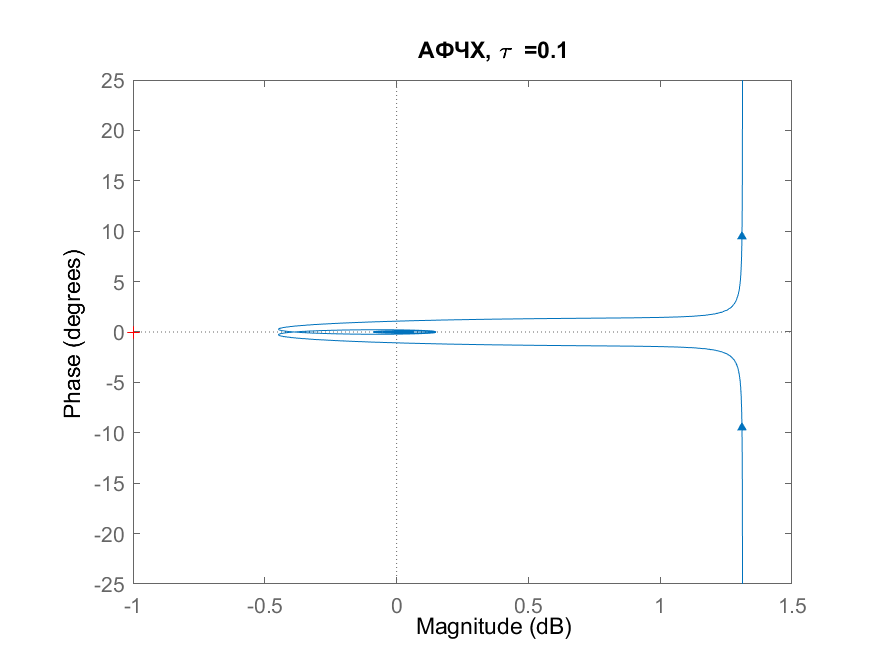
\includegraphics[width=0.7\textwidth]{nyquist_task32_object1.png}
    \caption{Годограф Найквиста для разомкнутой системы, $\tau=0.1$}
\end{figure}
\begin{figure}[ht]
    \centering
    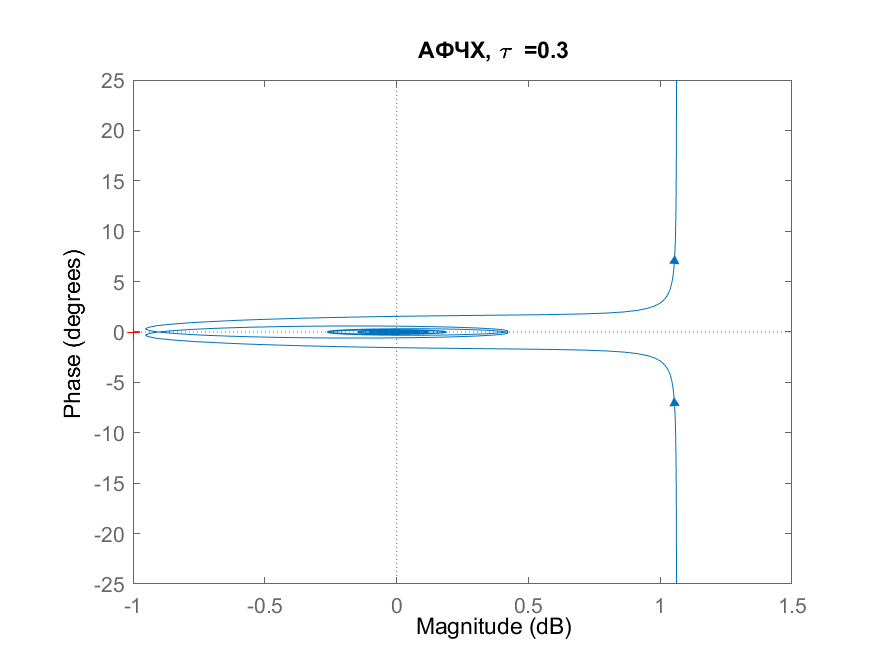
\includegraphics[width=0.7\textwidth]{nyquist_task33_object1.png}
    \caption{Годограф Найквиста для разомкнутой системы, $\tau=0.3$}
\end{figure}
\newpage
\begin{figure}[ht]
    \centering
    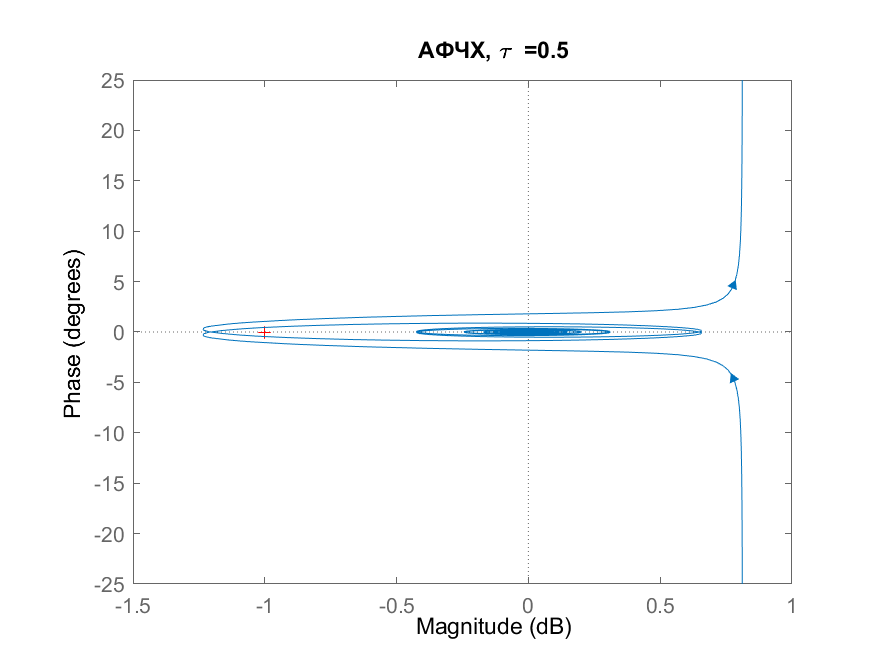
\includegraphics[width=0.7\textwidth]{nyquist_task34_object1.png}
    \caption{Годограф Найквиста для разомкнутой системы, $\tau=0.5$}
\end{figure}
\begin{figure}[ht]
    \centering
    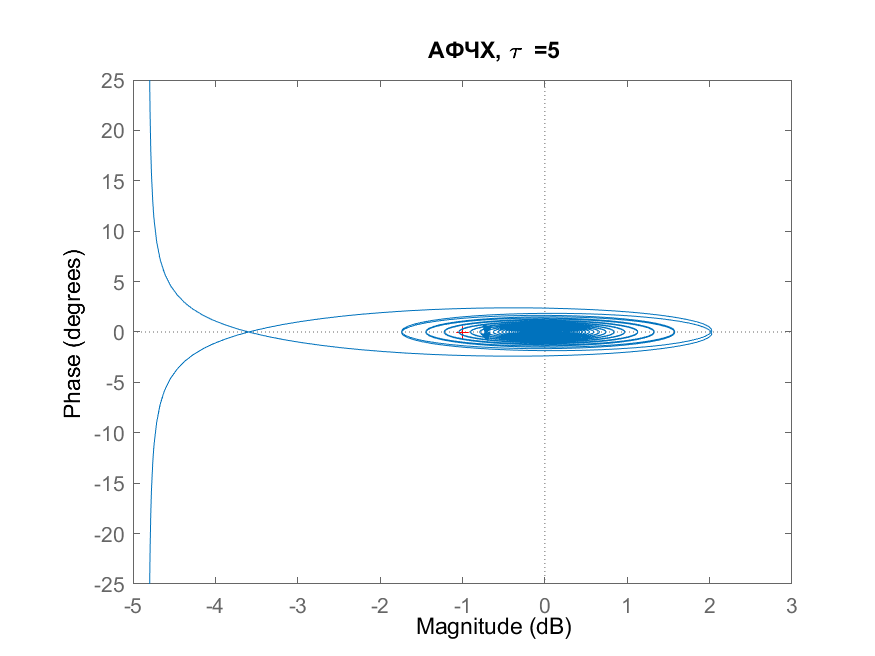
\includegraphics[width=0.7\textwidth]{nyquist_task35_object1.png}
    \caption{Годограф Найквиста для разомкнутой системы, $\tau=5$}
\end{figure}
\newpage
По полученным графикам можно заметить, что замкнутая система будет устойчива примерно до  $\tau< 0.4$, так как до $\tau < 0.3$ ещё всё хорошо и есть небольшой запас коэффицциента запаздывания. После же к системе прибавится два дополнительных неустойчивых полюсов, так как критическая точка попадёт внутрь годографа
и мы получим два оборота по часовой стрелке.

Давайте ниже узнаем точно диапазон - вычислим его аналитически\dots

\newpage
\subsection{Частотные характеристики}
Найдём критическое значение $\tau$. 

\begin{figure}[ht]
    \centering
    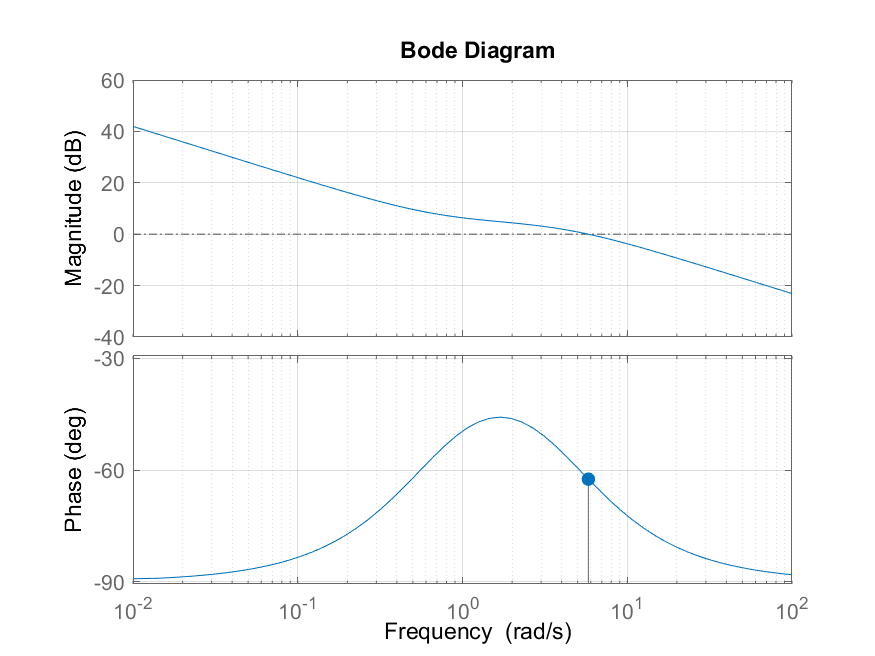
\includegraphics[width=0.7\textwidth]{log_nyquist_task3_object1.png}
    \caption{ЛАФЧХ, $\tau=5.0$}
\end{figure}
С помощью команды $\textrm{allmargin}$ получим информацию о критической точке на графике, её критическое значение и запас по фазе :
$$
 \tau_{crit} \approx 0.35, \tab \phi_3 \approx 117^\circ
$$

Теперь проверим аналитически, посчитаем $\tau_{crit}$, которые мы получили от \textit{matlab} до:
$$
\tau_{max} = \frac{\phi_3}{\omega_\phi}
$$, где $\phi_3$ - запас по фазе, $\omega_\phi$ - частота, соответствующая запасу по фазе. Эти два параметра мы можем найти для двух точек, если приблизим график достаточно точно, тогда получим:
$$
\tau_{crit} = \frac{117.54\pi}{180\cdot 5.8084} = 0.3537
$$

Как можно заметить, аналитически посчитанные совпали с ответами от \textit{allmargin}.


\newpage
\subsection{Переходные функции}
\begin{figure}[ht]
    \centering
    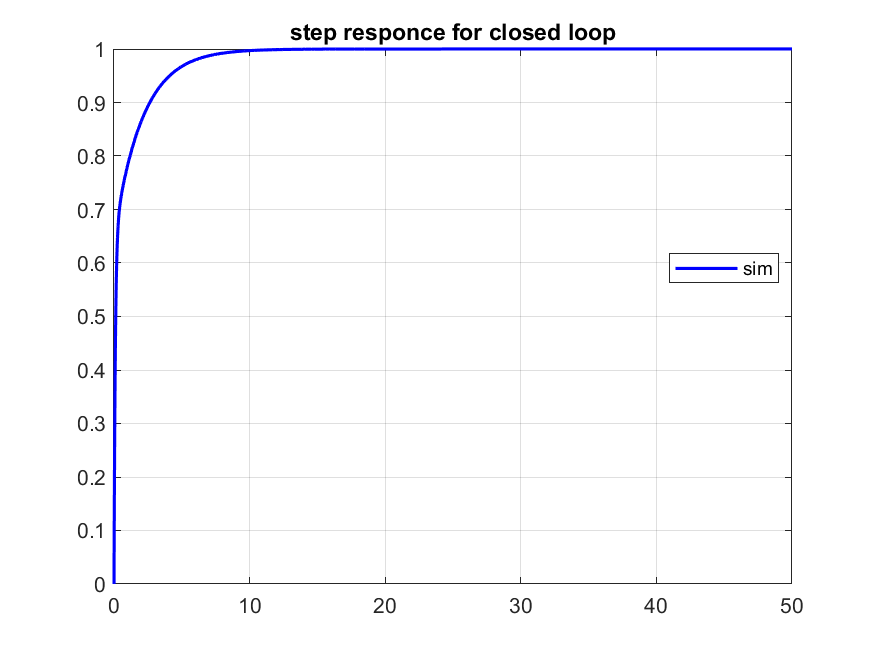
\includegraphics[width=0.7\textwidth]{step_responce31_closed1.png}
    \caption{Переходная функция для замкнутой системы, $\tau=0$}
\end{figure}
\begin{figure}[ht]
    \centering
    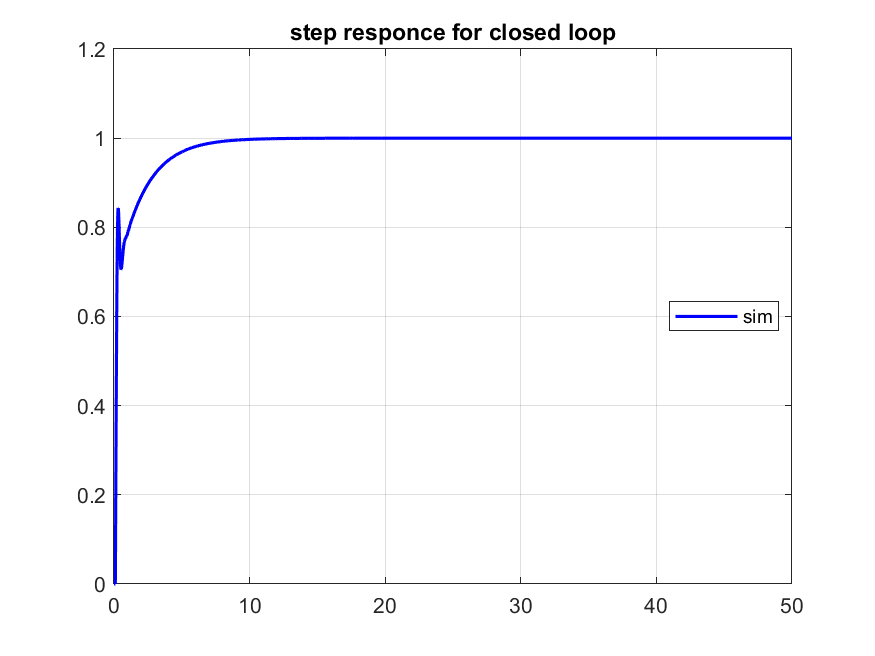
\includegraphics[width=0.7\textwidth]{step_responce32_closed1.png}
    \caption{Переходная функция для замкнутой системы, $\tau=0.1$}
\end{figure}

\newpage
\begin{figure}[ht]
    \centering
    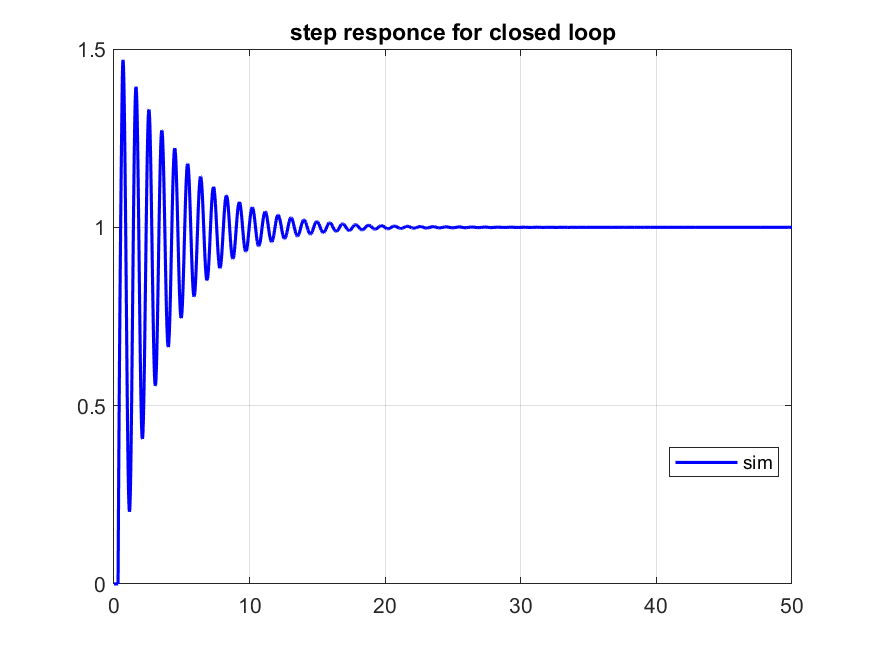
\includegraphics[width=0.7\textwidth]{step_responce33_closed1.png}
    \caption{Переходная функция для замкнутой системы, $\tau=0.3$}
\end{figure}
\begin{figure}[ht]
    \centering
    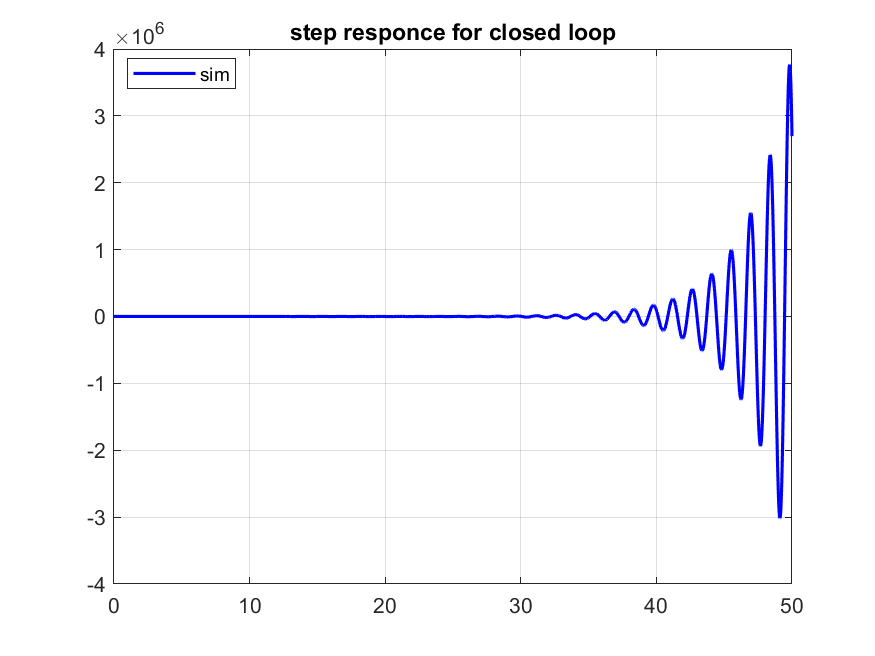
\includegraphics[width=0.7\textwidth]{step_responce34_closed1.png}
    \caption{Переходная функция для замкнутой системы, $\tau=0.5$}
\end{figure}
\newpage
\begin{figure}[ht]
    \centering
    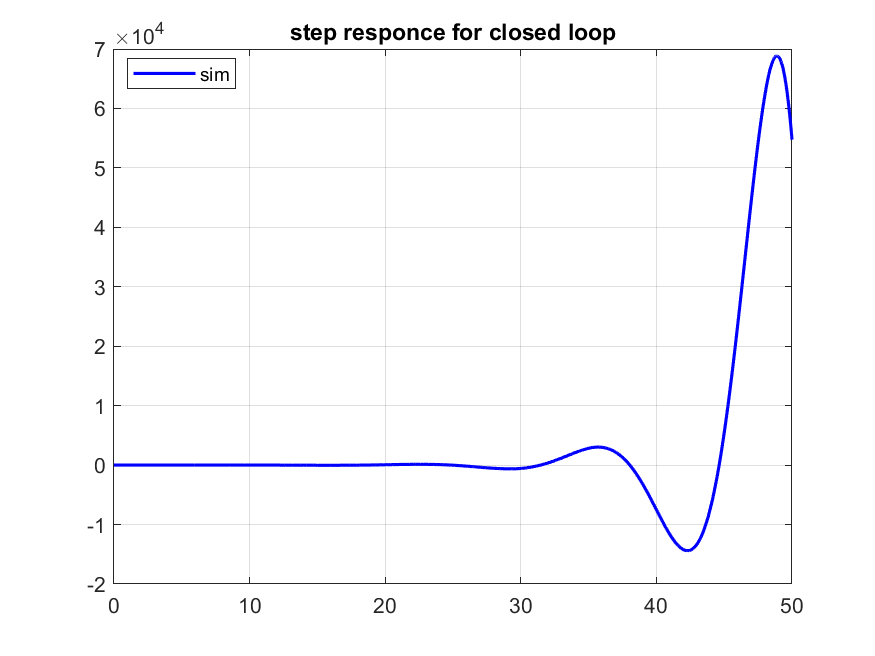
\includegraphics[width=0.7\textwidth]{step_responce35_closed1.png}
    \caption{Переходная функция для замкнутой системы, $\tau=5$}
\end{figure}
По графикам можно заметить, что аналитические выкладки подтвердились - замкнутая система устойчива будет устойчива лишь при $\tau < 0.35 $.


\section{Передаточная функция $W_4$}
Рассмотрим обновлённую ПФ:
$$
    W_4(s) = \frac{20s^2 +1.6s +2}{10s^3-10s^2-0.1s+0.1}e^{-\tau s}
$$
Получим её полюса: $\lambda_{1,2,3} \approx \{-0.23, 0.11 \pm 0.17j \}$, система имеет два неустойчивых и один устойчивых полюс.

Построим для неё годографы, с разными $\tau$:
\begin{figure}[ht]
    \centering
    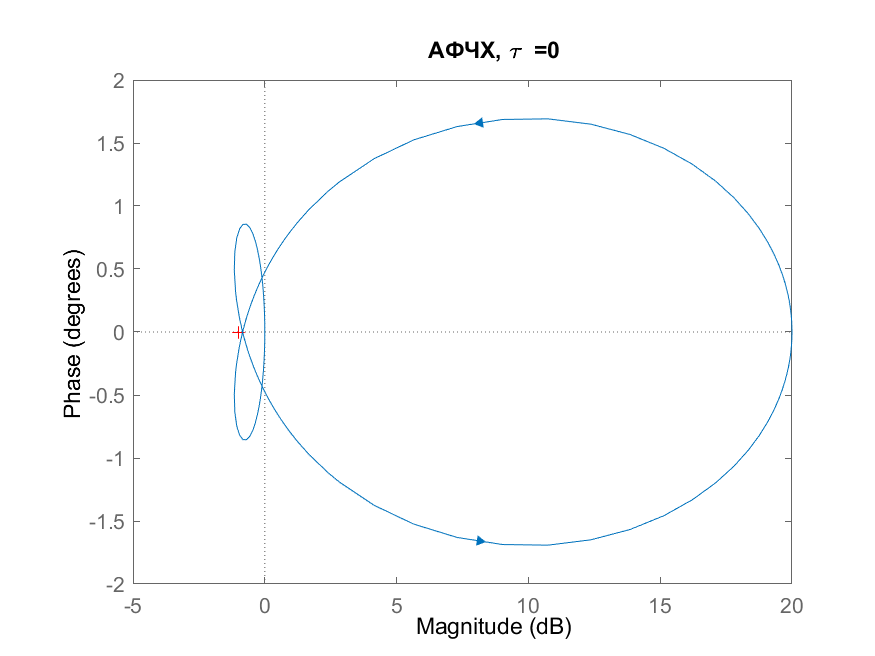
\includegraphics[width=0.7\textwidth]{nyquist_task31_object2.png}
    \caption{Годограф Найквиста для разомкнутой системы, $\tau=0$}
\end{figure}
\newpage
\begin{figure}[ht]
    \centering
    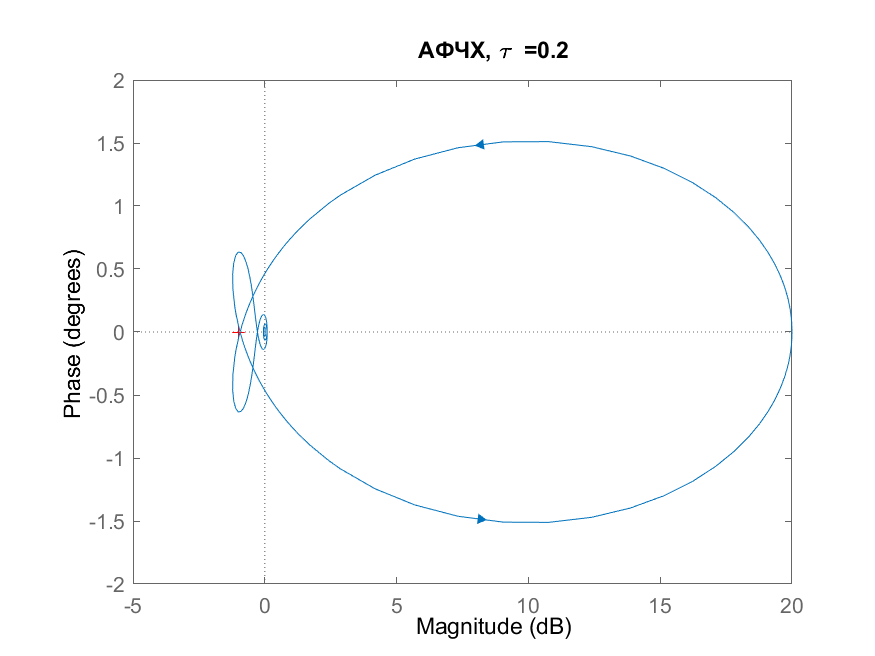
\includegraphics[width=0.7\textwidth]{nyquist_task33_object2.png}
    \caption{Годограф Найквиста для разомкнутой системы, $\tau=0.2$}
\end{figure}

\begin{figure}[ht]
    \centering
    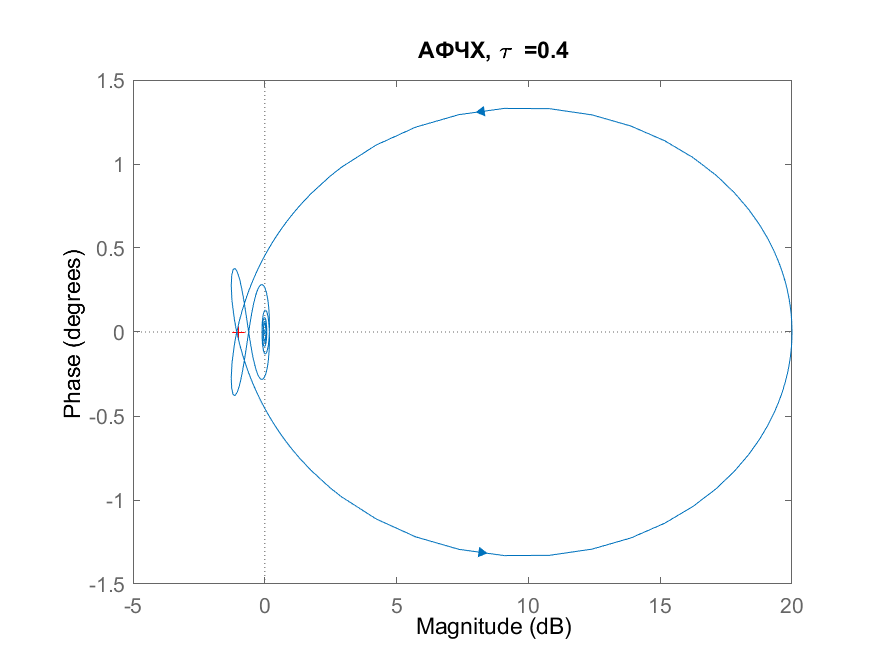
\includegraphics[width=0.7\textwidth]{nyquist_task35_object2.png}
    \caption{Годограф Найквиста для разомкнутой системы, $\tau=0.4$}
\end{figure}
\newpage
\begin{figure}[ht]
    \centering
    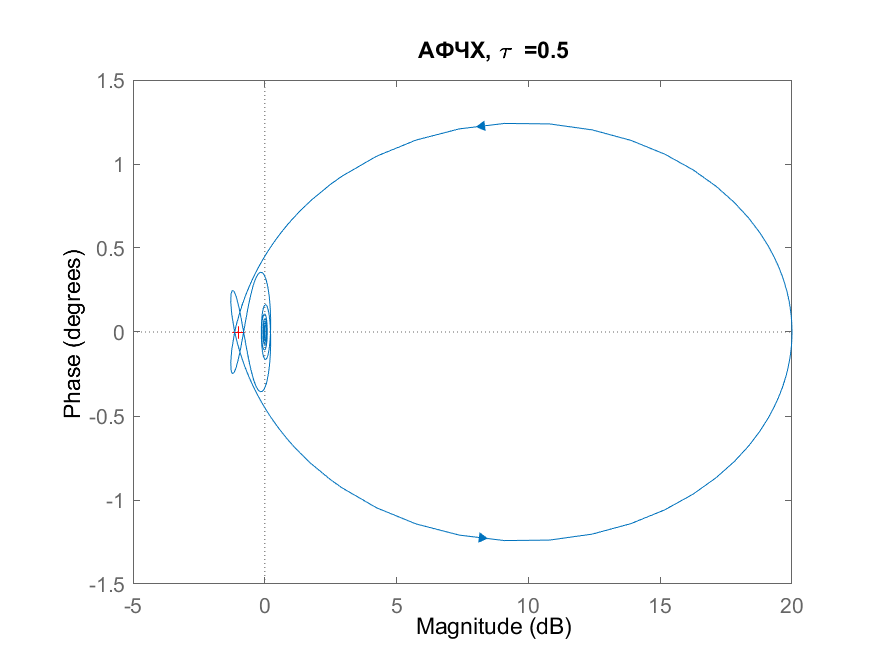
\includegraphics[width=0.7\textwidth]{nyquist_task36_object2.png}
    \caption{Годограф Найквиста для разомкнутой системы, $\tau=0.5$}
\end{figure}
\begin{figure}[ht]
    \centering
    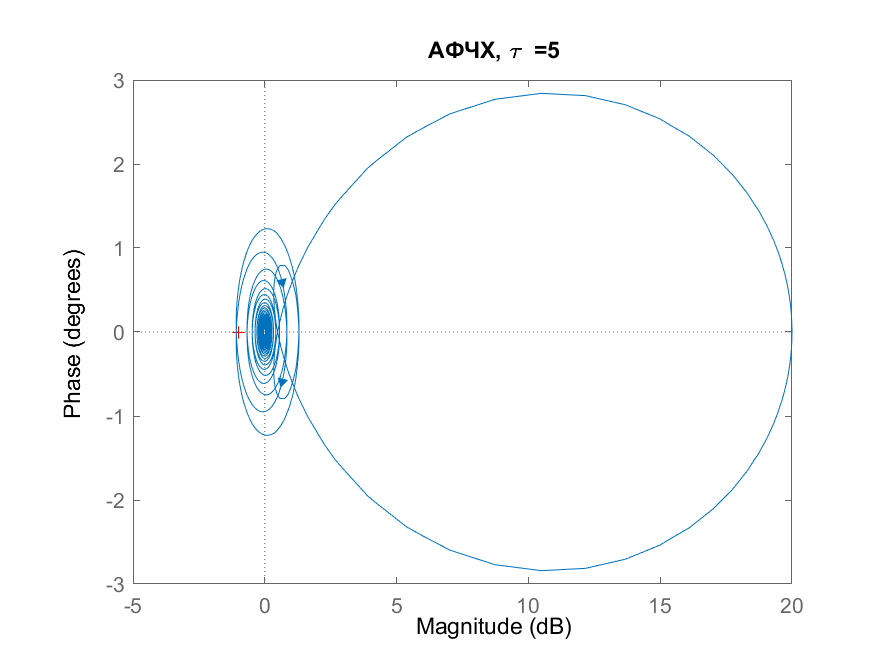
\includegraphics[width=0.7\textwidth]{nyquist_task39_object2.png}
    \caption{Годограф Найквиста для разомкнутой системы, $\tau=5$}
\end{figure}
\newpage
\begin{figure}[ht]
    \centering
    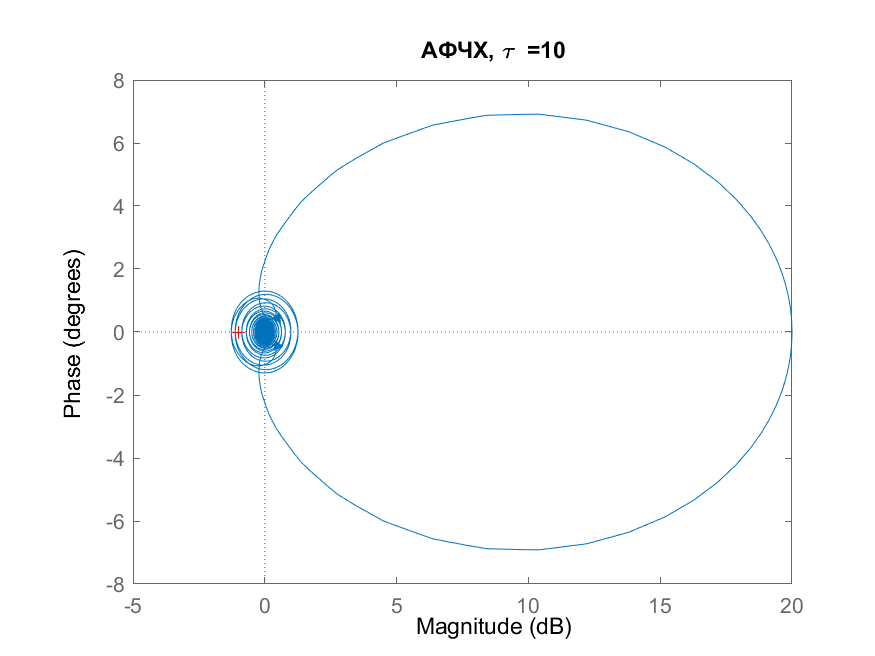
\includegraphics[width=0.7\textwidth]{nyquist_task310_object2.png}
    \caption{Годограф Найквиста для разомкнутой системы, $\tau=10$}
\end{figure}
По полученным графикам пока рано говорить об устойчивости в зависимости от задержки, потому что, например, примерно до $\tau< 0.3$ мы не получаем обороты, которые могут убрать нам неустойчивые полюса, а могут и прибавить, зависит от направления оборотов.
После же, при $\tau > 0.3$ пока рано о чём-либо заявлять, количество и направления трудно установить, поэтому лучше рассмотреть логарифмический критерий Найквиста и аналитически установить диапазон для $\tau$\dots

\newpage
\subsection{Частотные характеристики}
Попробуем найти критическое значение $\tau$. 

\begin{figure}[ht]
    \centering
    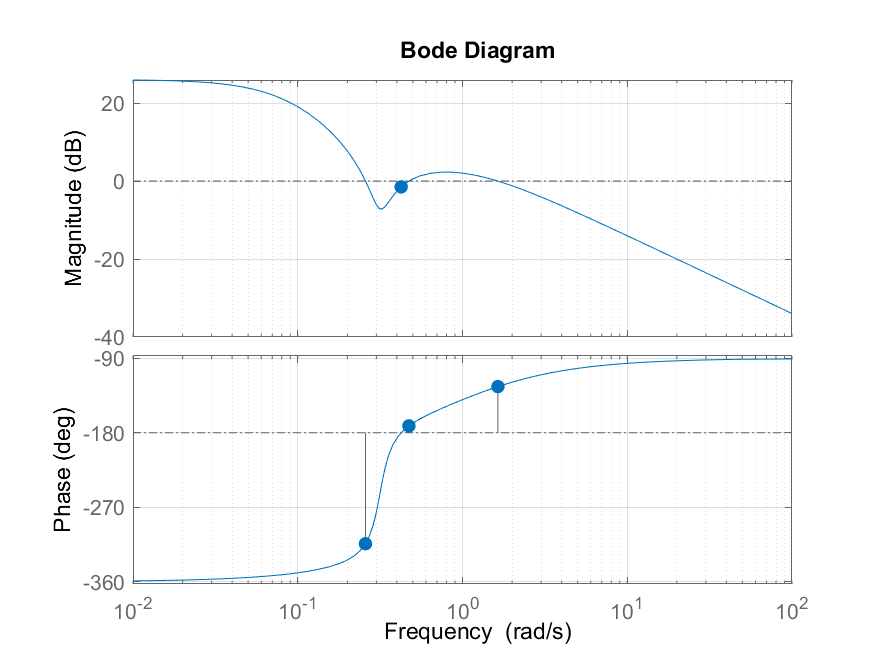
\includegraphics[width=0.7\textwidth]{log_nyquist_task3_object2.png}
    \caption{ЛАФЧХ, $\tau=5.0$}
\end{figure}

Однако всё же с помощью функции \textit{allmargin}  мы можем получить критическое допустимое время запаздывания и запас по фазе для этих точек:


$$
\begin{aligned}
    \tau_{crit1}=15.2, \tab \phi_{13}=-135^\circ, \\   
    \tau_{crit2}=0.3, \tab \phi_{23}=5.5^\circ, \\
    \tau_{crit3}=0.59, \tab \phi_{33}=46^\circ
\end{aligned}
$$

% Как можно заметить их будет три, но при проверке критерия можно заметить:
% нам нужно, чтобы сумма положительных и отриательных переходов через критический отрезок была равна $\frac{r}{2}= 1$. Но при $L(\omega) > 0$ у нас нет переходов, поэтому замкнутая система будет нейстойчивой. У системы не будет запаса устойчивости по фазе.

Как можно заметить, один из кандидатов на запас по фазе у нас отрицательный, поэтому его отбросим и сосредоточимся на двух оставшихся критических точках.

Давайте аналитически посчитаем $\tau_{crit2}, \tau_{crit3}$, которые мы получили от \textit{matlab} до:
$$
\tau_{max} = \frac{\phi_3}{\omega_\phi}
$$, где $\phi_3$ - запас по фазе, $\omega_\phi$ - частота, соответствующая запасу по фазе. Эти два параметра мы можем найти для двух точек, если приблизим график достаточно точно, тогда получим:
$$
\tau_{crit2} = \frac{8.26\pi}{180\cdot 0.4727} \approx 0.304 , \tab \tau_{crit3} = \frac{55.72\pi}{180\cdot 1.6401} \approx 0.59
$$
Получается, что замкнутая система устойчива будет устойчива в диапазоне между двумя критическими значениями, то есть: $\tau \in (0.304; 0.59)$.
Как можно заметить, аналитически посчитанные совпали с ответами от \textit{allmargin}. Проверим это на практике:

\newpage
\subsection{Переходные функции}
\begin{figure}[ht]
    \centering
    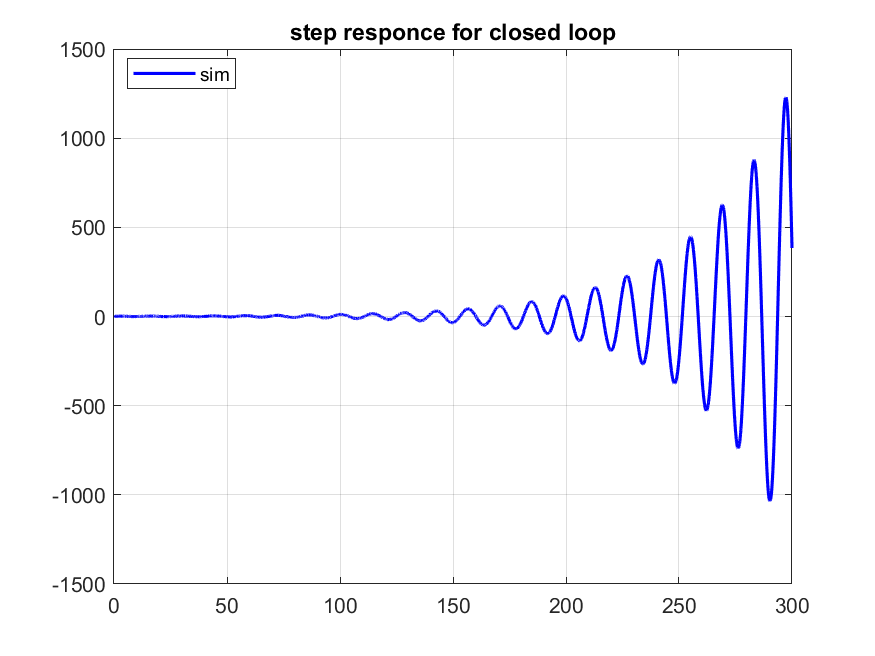
\includegraphics[width=0.7\textwidth]{step_responce31_closed2.png}
    \caption{Переходная функция для замкнутой системы, $\tau=0$}
\end{figure}
\begin{figure}[ht]
    \centering
    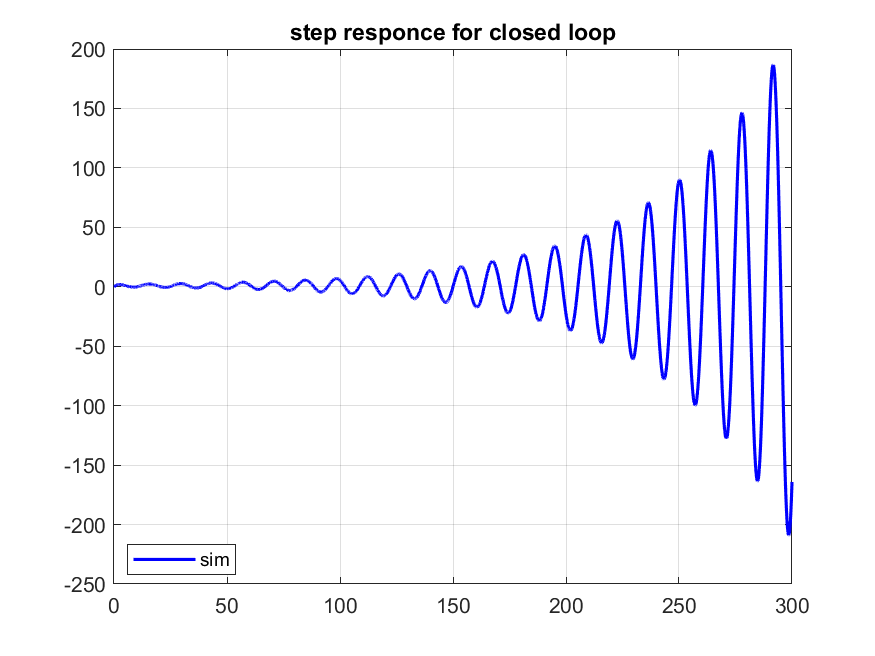
\includegraphics[width=0.7\textwidth]{step_responce32_closed2.png}
    \caption{Переходная функция для замкнутой системы, $\tau=0.1$}
\end{figure}

\newpage
\begin{figure}[ht]
    \centering
    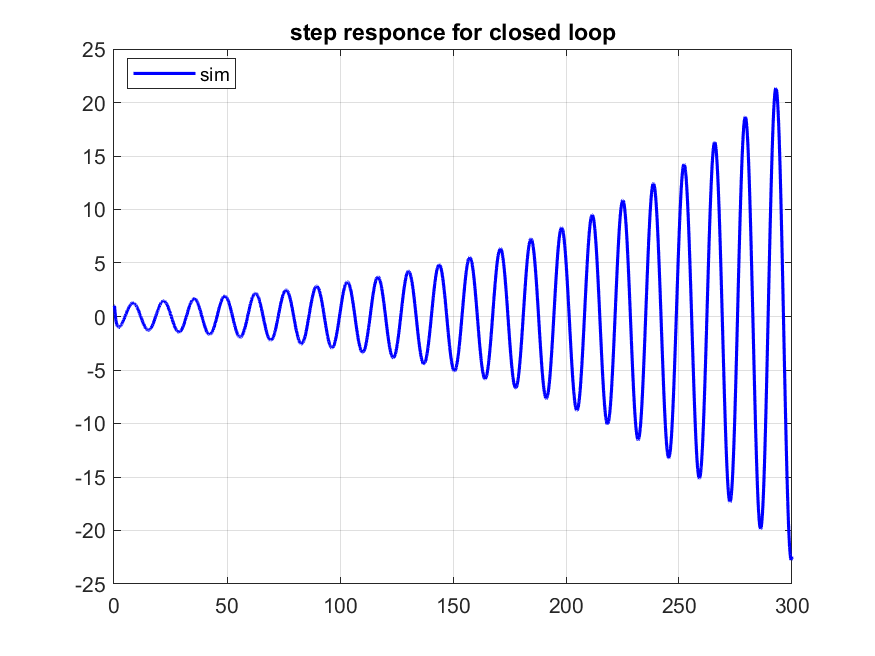
\includegraphics[width=0.7\textwidth]{step_responce33_closed2.png}
    \caption{Переходная функция для замкнутой системы, $\tau=0.2$}
\end{figure}
\begin{figure}[ht]
    \centering
    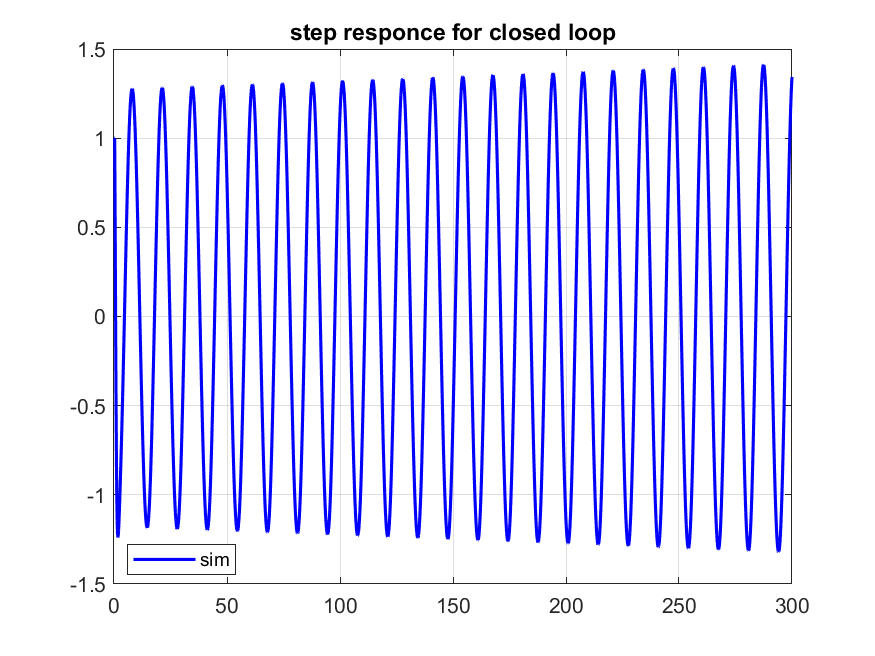
\includegraphics[width=0.7\textwidth]{step_responce34_closed2.png}
    \caption{Переходная функция для замкнутой системы, $\tau=0.3$}
\end{figure}

\newpage
\begin{figure}[ht]
    \centering
    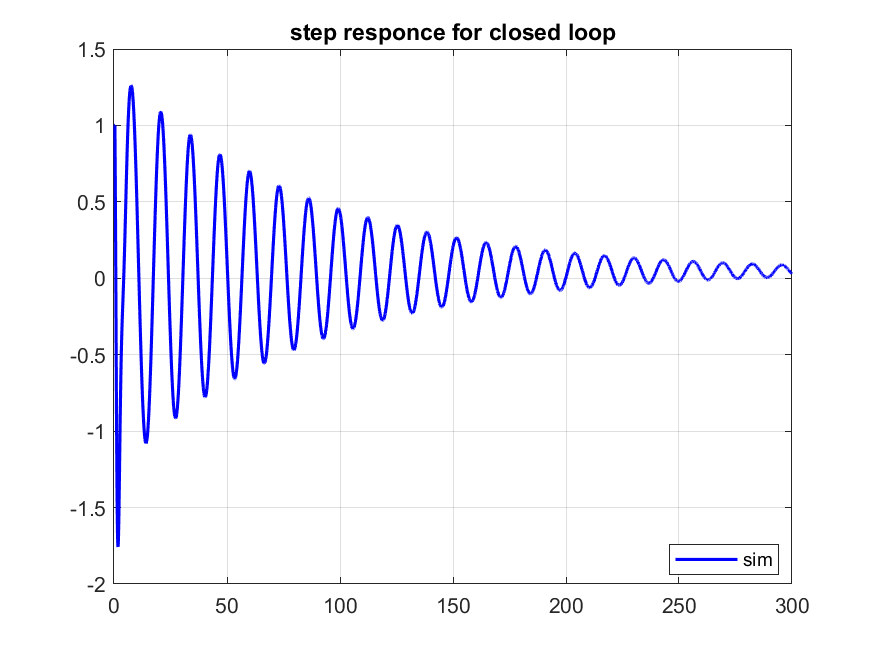
\includegraphics[width=0.7\textwidth]{step_responce35_closed2.png}
    \caption{Переходная функция для замкнутой системы, $\tau=0.4$}
\end{figure}
\begin{figure}[ht]
    \centering
    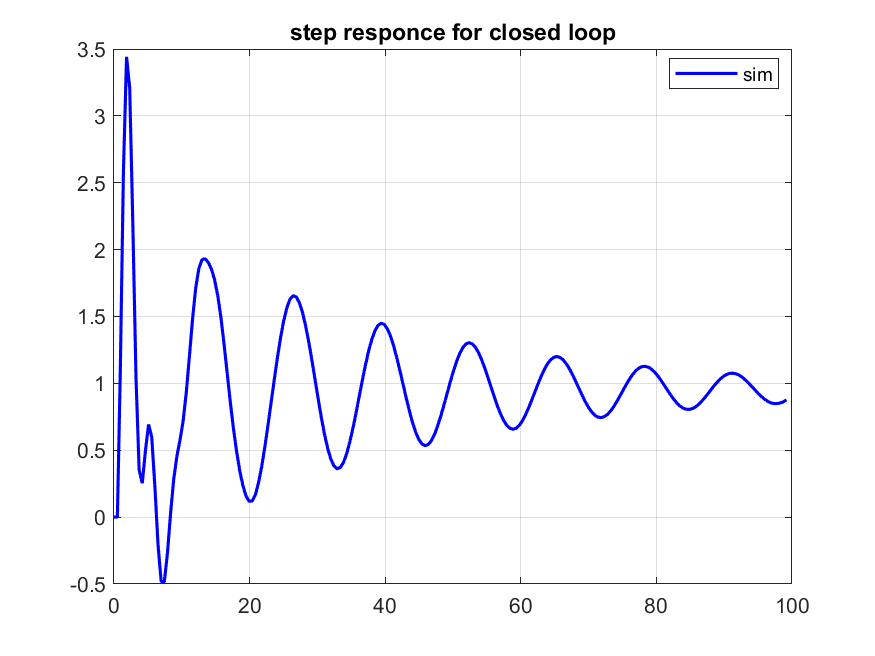
\includegraphics[width=0.7\textwidth]{step_responce36_closed2.png}
    \caption{Переходная функция для замкнутой системы, $\tau=0.5$}
\end{figure}

\newpage
\begin{figure}[ht]
    \centering
    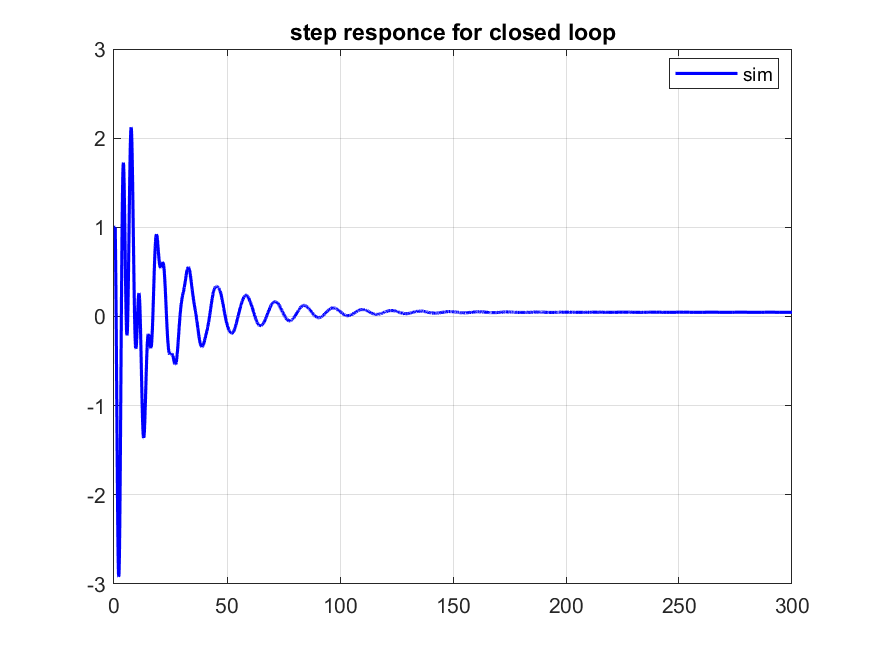
\includegraphics[width=0.7\textwidth]{step_responce37_closed2.png}
    \caption{Переходная функция для замкнутой системы, $\tau=0.55$}
\end{figure}
\begin{figure}[ht]
    \centering
    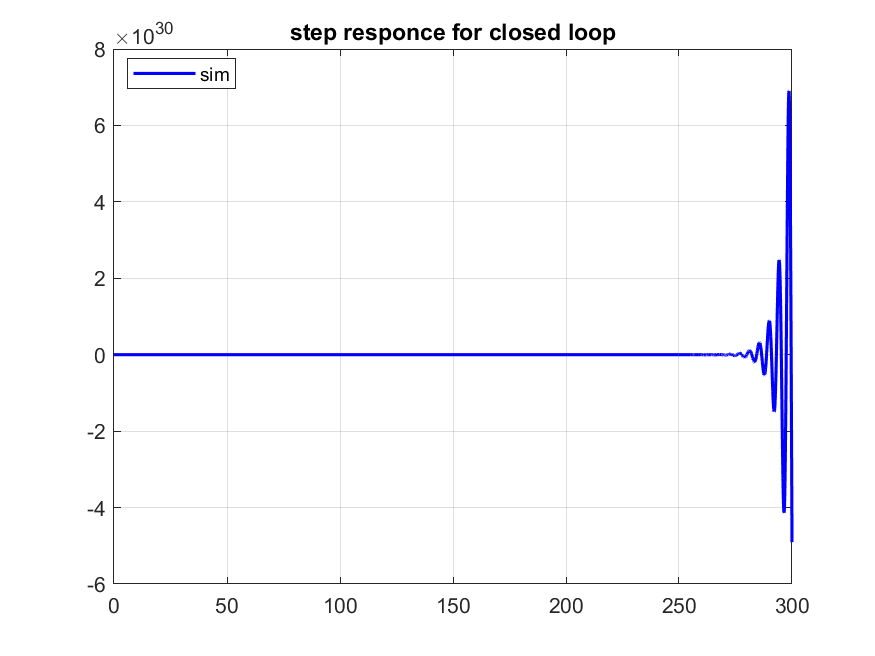
\includegraphics[width=0.7\textwidth]{step_responce38_closed2.png}
    \caption{Переходная функция для замкнутой системы, $\tau=0.7$}
\end{figure}

\newpage
\begin{figure}[ht]
    \centering
    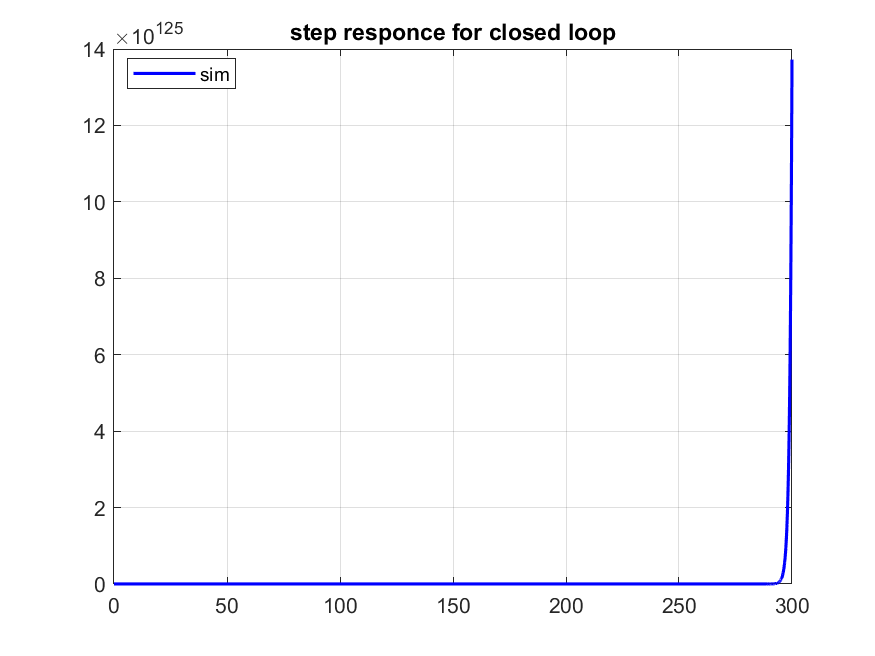
\includegraphics[width=0.7\textwidth]{step_responce39_closed2.png}
    \caption{Переходная функция для замкнутой системы, $\tau=5$}
\end{figure}
\begin{figure}[ht]
    \centering
    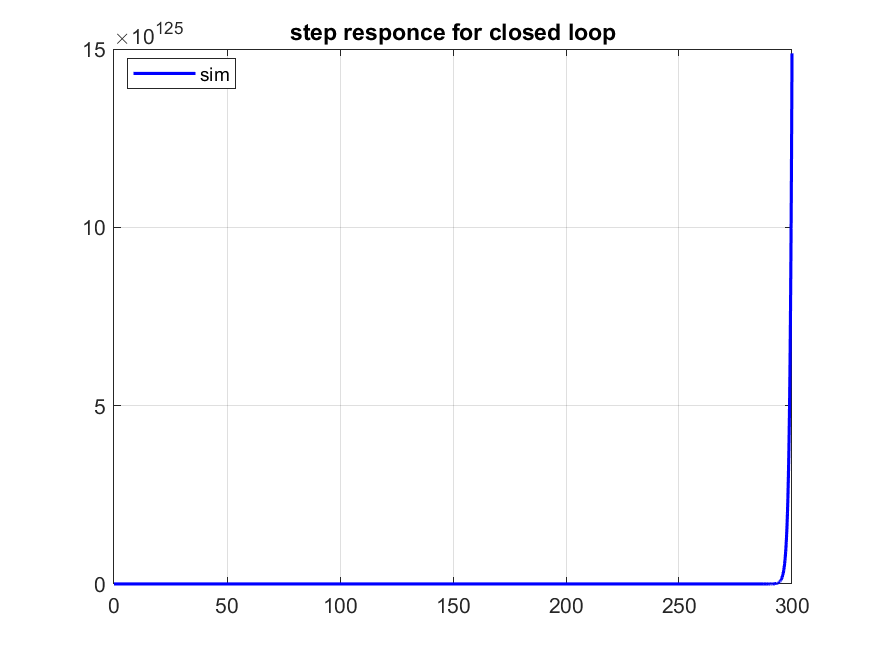
\includegraphics[width=0.7\textwidth]{step_responce310_closed2.png}
    \caption{Переходная функция для замкнутой системы, $\tau=10$}
\end{figure}

По графикам можно заметить, что аналитические выкладки подтвердились - замкнутая система устойчива будет устойчива при $\tau \in (0.304; 0.59)$.

\endinput